
\documentclass[paper=a4, fontsize=11pt]{scrartcl} % A4 paper and 11pt font size

\usepackage[T1]{fontenc} % Use 8-bit encoding that has 256 glyphs
\usepackage{fourier} % Use the Adobe Utopia font for the document - comment 
\usepackage[english]{babel} % English language/hyphenation
\usepackage{amsmath,amsfonts,amsthm} % Math packages
\usepackage{graphicx}
\usepackage{float}
\usepackage{subfig}
\usepackage{caption}
\usepackage[section]{placeins}
\usepackage{sectsty} % Allows customizing section commands
\allsectionsfont{\centering \normalfont\scshape} 
\numberwithin{equation}{section} 
\numberwithin{figure}{section} 
\numberwithin{table}{section} 

\setlength\parindent{2pt} 
%-------------------------------------------------------------------------------
%	TITLE SECTION
%-------------------------------------------------------------------------------

\newcommand{\horrule}[1]{\rule{\linewidth}{#1}} 

\title{	
\normalfont \normalsize 
\textsc{PH 481 Lab} \\ [25pt] 
\horrule{2pt} \\[0.5cm] % Thin top horizontal rule
\huge Optics Lab 8\\ % The assignment title
\horrule{2pt} \\[0.5cm] % Thick bottom horizontal rule
}

\author{Harsukh Singh} % Your name

\date{\normalsize \today} % Today's date or a custom date

\begin{document}

\maketitle % Print the title
\section{Overview of Experiment}
This experiment involved the study of Birefringence and its effect on polarization of an electromagnetic wave.
\section{Birefringence and Optical Isolation}
 In this study, we aligned the laser to the Optical Rail per usual and then inserted a quarter wave plate in the optical rail. A quarter-wave plate is designed so that the fast and slow components of a wave will experience a relative phase shift of $\frac{\pi}{2}$. Thus the wave is circularly polarized. {\bfseries This can be checked if another polarizer is placed in front the quarter wave plate, the total amplitude of the wave remains unchanged; $\vec{E} \cdot \vec{E}$ is constant regardless of the orientation of the polarizer.}The set up for the experiment is  shown in Figure ~\ref{fig:stage}. 
 
\begin{figure}[H]
\centering
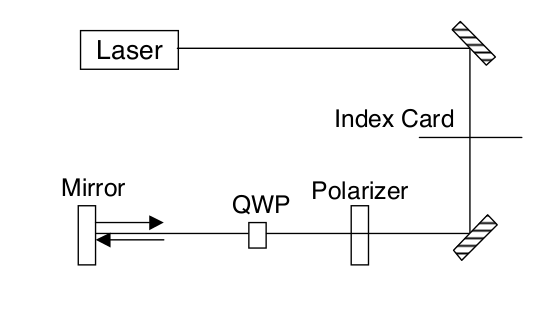
\includegraphics[scale =0.4]{stage}
\caption{Experimental Set Up}
\label{fig:stage}
\end{figure}

With this setup we used the mirror at the end of the optical rail (after the retarder), to slightly relfect the beam so it was distinguishable from the incoming beam. Then we rotated the quarter wave plate until the reflected beam was minimized after this was done we varied the angle of incidence until the the reflected beam completely disappeared. Thus this completed the build of the optical isolator. \\

Once this was done. We changed orientation of the light to normal incidence and found two positions that produced circularly polarized light. This happens because the wave has to be $45^{\circ}$ to the horizontal or $315^{\circ}$. Addition of two quarter wave plates make a half wave plate, if the incoming light is in the $\mathcal{P}$-state then the handedness of the light just flips.
\section{Birefringent Crystals}
The Birefringence of the crystal is defined by the quantity $\Delta n = (n_e-n_o)$  where e and o are the extraordinary and oridnary indices of refraction. Any natural light coming from these crystals give rise to spherical o-wavelets and ellipsoidal e-wavelets. The E field of the o-wave is normal to the optical axis everywhere and the addition of the polarizer removes the effect of the additional e-waves. Thus only allowing the o-wavelets through.
\section{Optical Activity}
In this section we explored the optical activity in a material.  In this case, we explored a sugar solution. We set the solution at a concentration of solution to, $c_0 = 1 \frac{g}{ml}$ and put it onto the optical rail with a polarizer and analyzer and minimzed the light coming out of the solution. With this we want our observations to be consistent with sugar being dextrorotary, so we want to check the equation,

\begin{equation}
d\times c\times [\alpha]_{\lambda}^T = \beta
\end{equation}

Where $\beta$ is the angle of rotation and d is the diameter of liquid which was measured to be 7.35 cm. c is the concentration and alpha is the specific rotation given by, 
$+66.5 \frac{degrees/dm}{g/ml}$

We vary the concentration to plot and see if the law holds (see if it's a linear fit). The results are shown in figure ~\ref{fig:figure}, we find the specific rotation to be $+49.1 \frac{degrees/dm}{g/ml}$ as shown by the graph. It would have helped to taken more data points.

\begin{figure}[H]
\centering
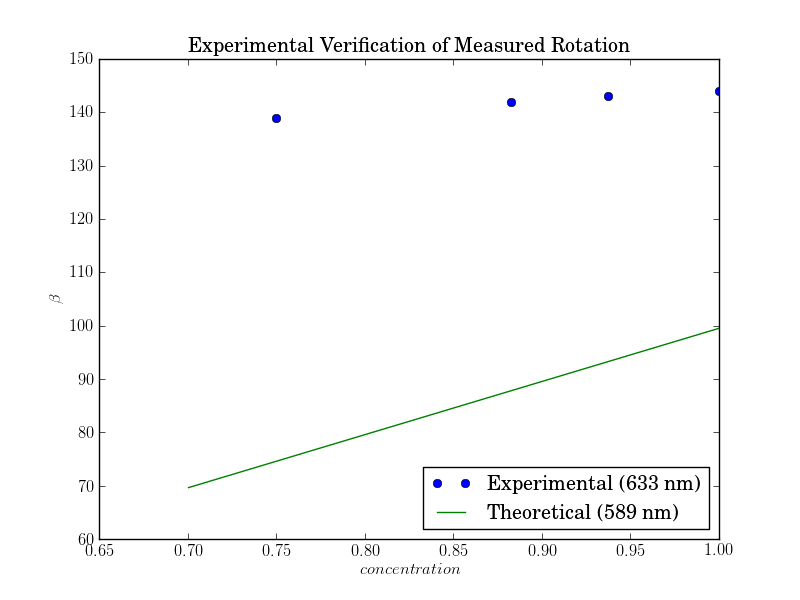
\includegraphics[scale =0.4]{fig}
\caption{Theoretical and Experimental Plot}
\label{fig:figure}
\end{figure}

\section{Conclusion}
This lab studied the effect and properties of birefringent materials. There may be some uncertainty involved in the collection of data seen in figure ~\ref{fig:figure}. For example the calculation of the slope needs more data points for the least squares algorithm to be entirely accurate.

\end{document}


%\begin{figure}[htb]
%\centering
%\parbox{5cm}{
%\includegraphics[width=5cm]{figure_1}
%\caption{ Reflection Coefficients}}
%\qquad
%\begin{minipage}{5cm}
%\includegraphics[width=5cm]{figure_2}
%\caption{Transmission Coefficients}
%\end{minipage}
%\end{figure}
%
%\begin{figure}[htb]
%\centering
%\parbox{5cm}{
%\includegraphics[width=5cm]{Epar}
%\caption{Electric Field Parallel to Incident Plane}
%\label{fig:2figsA}}
%\qquad
%\begin{minipage}{5cm}
%\includegraphics[width=5cm]{Eperp}
%\caption{Electric Field Perpendicular to Indicent Plane}
%\label{fig:2figsB}
%\end{minipage}
%%\end{figure}
%
%\section{Experiment 1.1:  Transmittance through Glass}
%\begin{figure}[!ht]
%	\caption{Experimental Set-Up}
%		\begin{center}
%			\includegraphics[scale=0.5]{transmittance}
%		\end{center}
%\end{figure}

%\begin{figure}[!ht]
%	\caption{Experimental Comparison to Theoretical Transmission 
%Coefficients}
%		\begin{center}
%			\includegraphics[scale=0.5]{figure_3}
%		\end{center}
%\end{figure}
%
%\section{Experiment 1.2:  Reflectance from Frosted Glass}
%\begin{figure}[!ht]
%		\begin{center}
%			\includegraphics[scale=0.5]{reflectance}
%		\end{center}
%\caption{Reflectance from Frosted Glass}
%\end{figure}

%\section{Experiment 1.3: Refraction through glass slab}
%\begin{figure}[!ht]
%		\begin{center}
%			\includegraphics[scale=0.5]{GlassLab}
%		\end{center}
%\caption{Measuring the index of refraction through Glass Slab}
%\end{figure}g
% \begin{equation}
%sin(\theta_i -\theta_t) = \frac{l}{\frac{t}{cos(\theta_t)}}
% \end{equation}
% and,
% \begin{equation}
%n_{slab}  = 
%\frac{n_1sin(\theta_1)}{sin(\theta_1-sin^{-1}(\frac{t}{\frac{l}{sin(\theta_i 
%-\theta_t)}}))}
% \end{equation}
% Solving this $n_{slab} = 1.42$  and since most glass has a refractive index 
% of ~1.5 this was pretty close.
% \begin{equation}
%   \begin{tabular}{|l |r| }
%     \hline
%      d(m) & 0.0065561             \\ \hline
%     d^{'} (m) & 0.0064660        \\ \hline
%     d^{''}(m) & 0.006345             \\  \hline
%     d^{'''}(m)& 0.0061452               \\  \hline
%   \end{tabular}
% \end{equation}
% \begin{figure}[htb]
% 	\caption{Fabry-Perot fringes (I vs delta)}
% 		\begin{center}
% 			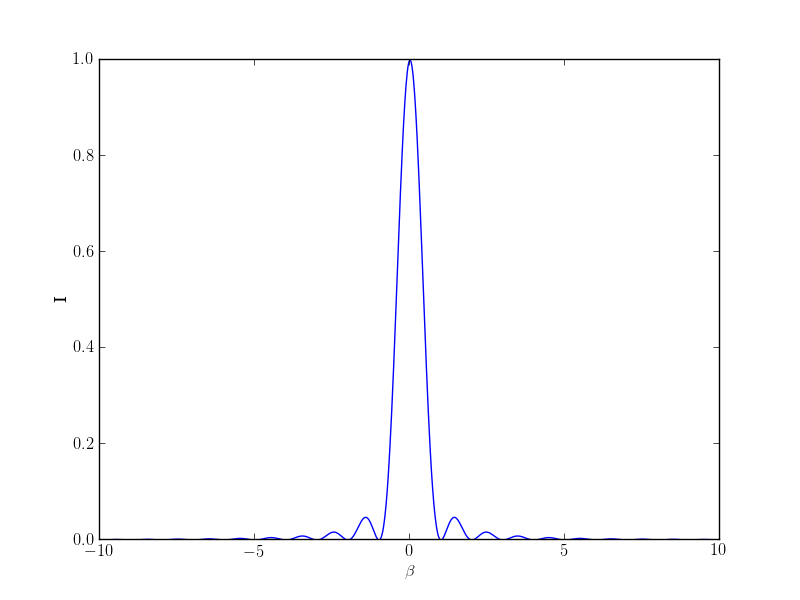
\includegraphics[scale=0.5]{fringes}
% 		\end{center}
% \end{figure}
% \begin{table}[H]
%   \centering 
%    \caption{data}
%   \begin{tabular}{|l |r| }
%     \hline
%      3 slits & $\frac{2}{3}$ \\ \hline
%      4 slits & $\frac{2}{4}$ \\ \hline
%      10 slits & $\frac{2}{3}$ \\  \hline
%   \end{tabular}
% \end{table}
% \begin{figure}[H]
% \centering
% 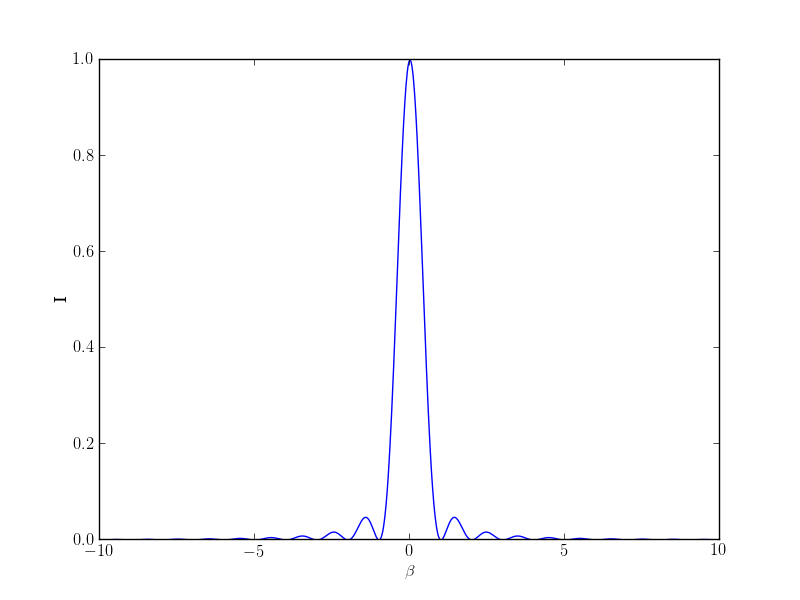
\includegraphics[scale =0.4]{fringes}
% \caption{Irradiance}
% \end{figure}
